%%%%%%%%%%%%%%%%%%%%%%%%%%%%%%%%%%%%%%%%%%%%%%%%%%%%%%%%%%%%%%%%%%%%%%
%% Copyright waiver
%%%%%%%%%%%%%%%%%%%%%%%%%%%%%%%%%%%%%%%%%%%%%%%%%%%%%%%%%%%%%%%%%%%%%%

\documentclass{beamer}
\usetheme[faculty=econ]{fibeamer}

\usepackage{booktabs}
\usepackage{multirow}
\usepackage[nodayofweek]{datetime}
\usepackage{zed-csp}

\newdateformat{mydate}{\twodigit{\THEDAY}{ }\shortmonthname[\THEMONTH], \THEYEAR}

\makeatletter
\renewcommand\fibeamer@includeLogo[1][]{}
\makeatother

\usepackage[utf8]{inputenc}
\usepackage[main=english, czech]{babel}

\usepackage{ragged2e}
\usepackage{booktabs}
\usepackage{tabularx}
\usepackage{tikz}
\usetikzlibrary{calc, shapes, backgrounds}
\usepackage{amsmath, amssymb}
\usepackage{url}
\usepackage{listings}

\newlength{\myMheight}
\settoheight{\myMheight}{M}

\usepackage{scalerel}

\frenchspacing

\title{Overview of Research and Expertise\\
UCL School of Management
}
\subtitle{King's College London}
\author{Wenbin Wu\\ \today}

\begin{document}
\shorthandoff{-}
\frame[c]{\maketitle}

\AtBeginSection[]{%
\begin{frame}<beamer>
\frametitle{Outline}
\tableofcontents[currentsection]
\end{frame}}

\section{Self Introduction}

% Frame for the introduction
\begin{frame}{Self Introduction}
\framesubtitle{Wenbin Wu}
    \begin{itemize}
        \item \textbf{Current Research Focus}
        \begin{itemize}
            \item Computational finance and DeFi using agent-based modeling.
        \end{itemize}

        \item \textbf{Specialization}
        \begin{itemize}
            \item Price stability mechanisms of on-chain collateralized stablecoins.
        \end{itemize}

        \item \textbf{Experience}
        \begin{itemize}
            \item ABM simulation and sensitivity analysis. 
            \item Large scale stylized on-chain data analysis.
            \item Formal verification.
        \end{itemize}
    \end{itemize}
\end{frame}

% Frame for Education background
\begin{frame}{Education}
\framesubtitle{Wenbin Wu}
\begin{itemize}
\item \textbf{King’s College London}
\begin{itemize}
\item PhD in Computer Science
\item MSc Banking and Finance
\end{itemize}

\item \textbf{Peking University}
\begin{itemize}
\item MS Computational Finance
\end{itemize}

\item \textbf{University of Electronic Science and Technology of China}
\begin{itemize}
\item BSc Information Security
\end{itemize}
\end{itemize}
\end{frame}

\section{Current work}

\begin{frame}{PhD Research}
\framesubtitle{Background and Question}

\begin{itemize}
\item \textbf{Background}
\begin{itemize}

\item Stablecoin is a type of decentralized cryptocurrency.
\item Many stablecoins have experienced bank runs. 
\item Some encoutered outright collapse, e.g., Terra 
\includegraphics[height=1.2\myMheight]{resources/terra.png} and Basis 
\includegraphics[height=1.2\myMheight]{resources/basis.jpg}. 
\end{itemize}
\item \textbf{Question}
\begin{itemize}
\item What stablization policies improve price stability?
\item What is the implication of this?
\end{itemize}
\end{itemize}
\end{frame}

\begin{frame}{PhD Research}
\framesubtitle{Methods and Findings}

\begin{itemize}
\item \textbf{Methods}
\begin{itemize}
\item Analysis of stylized blockchain data and smart contracts.
\item ABM simulation. 
\item Some formal verification for the modeled stablecoin system.
\end{itemize}

\item \textbf{Findings}
\begin{itemize}
\item Two key parameters are most notable, \textcolor{red}{collateralization ratio} and \textcolor{red}{auction discount curve}.
\item High collateralization helps reduce irrational runs, and a steep discount curve limits the damage of rational runs. 
\item Runs are inevitable. Many on-chain stablecoins are taking up risky or dubious assets.  
\end{itemize}
\end{itemize}
\end{frame}


\begin{frame}{Collaboration}
\framesubtitle{Professional Collaborations and Roles}
\begin{itemize}
\item \textbf{Cambridge Center for Alternative Finance}
\begin{itemize}
    \item Collaborating DeFi mapping tools and panels.
    \item Analyzing granular real-time smart contract data.
    \item Providing insights on the DeFi landscape. 
\end{itemize}
\item \textbf{SoCityDAO and MIT Media Lab}
\begin{itemize}
\item Collaborating on carbon credit stablecoin.
\item Designing token framework.
\end{itemize}
\item \textbf{School of Economics, Peking University}
\begin{itemize}
\item Chinese CBDC under the guidance of a leading economist.
\item Contributed to conference presentations and policy briefs.
\end{itemize}
\end{itemize}
\end{frame}


\section{Future Plans}

\begin{frame}{Highlights}
\begin{itemize}
\item Cryptocurrency and Blockchain Research
\item Interdisciplinary experience intersecting with financial policy
\item Experience with applications of  
\item Tools: 
\begin{itemize}
    \item Python and NetLogo for agent-based modeling
    \item Python (\textcolor{red}{joblib} for multip), R, and SQL for financial statistics
    \item Solidity, Infura, and Web3 for blockchain integration
    \item BigQuery, AWS, streamlit, D3.js for data ETL and visualization
    \item Experience with writing collaborative and maintainable code 
\end{itemize}
\end{itemize}
\end{frame}




\begin{frame}{Thank you}

\end{frame}

\begin{frame}{Appendix: Some Stylized Data}
\begin{figure}
\centering
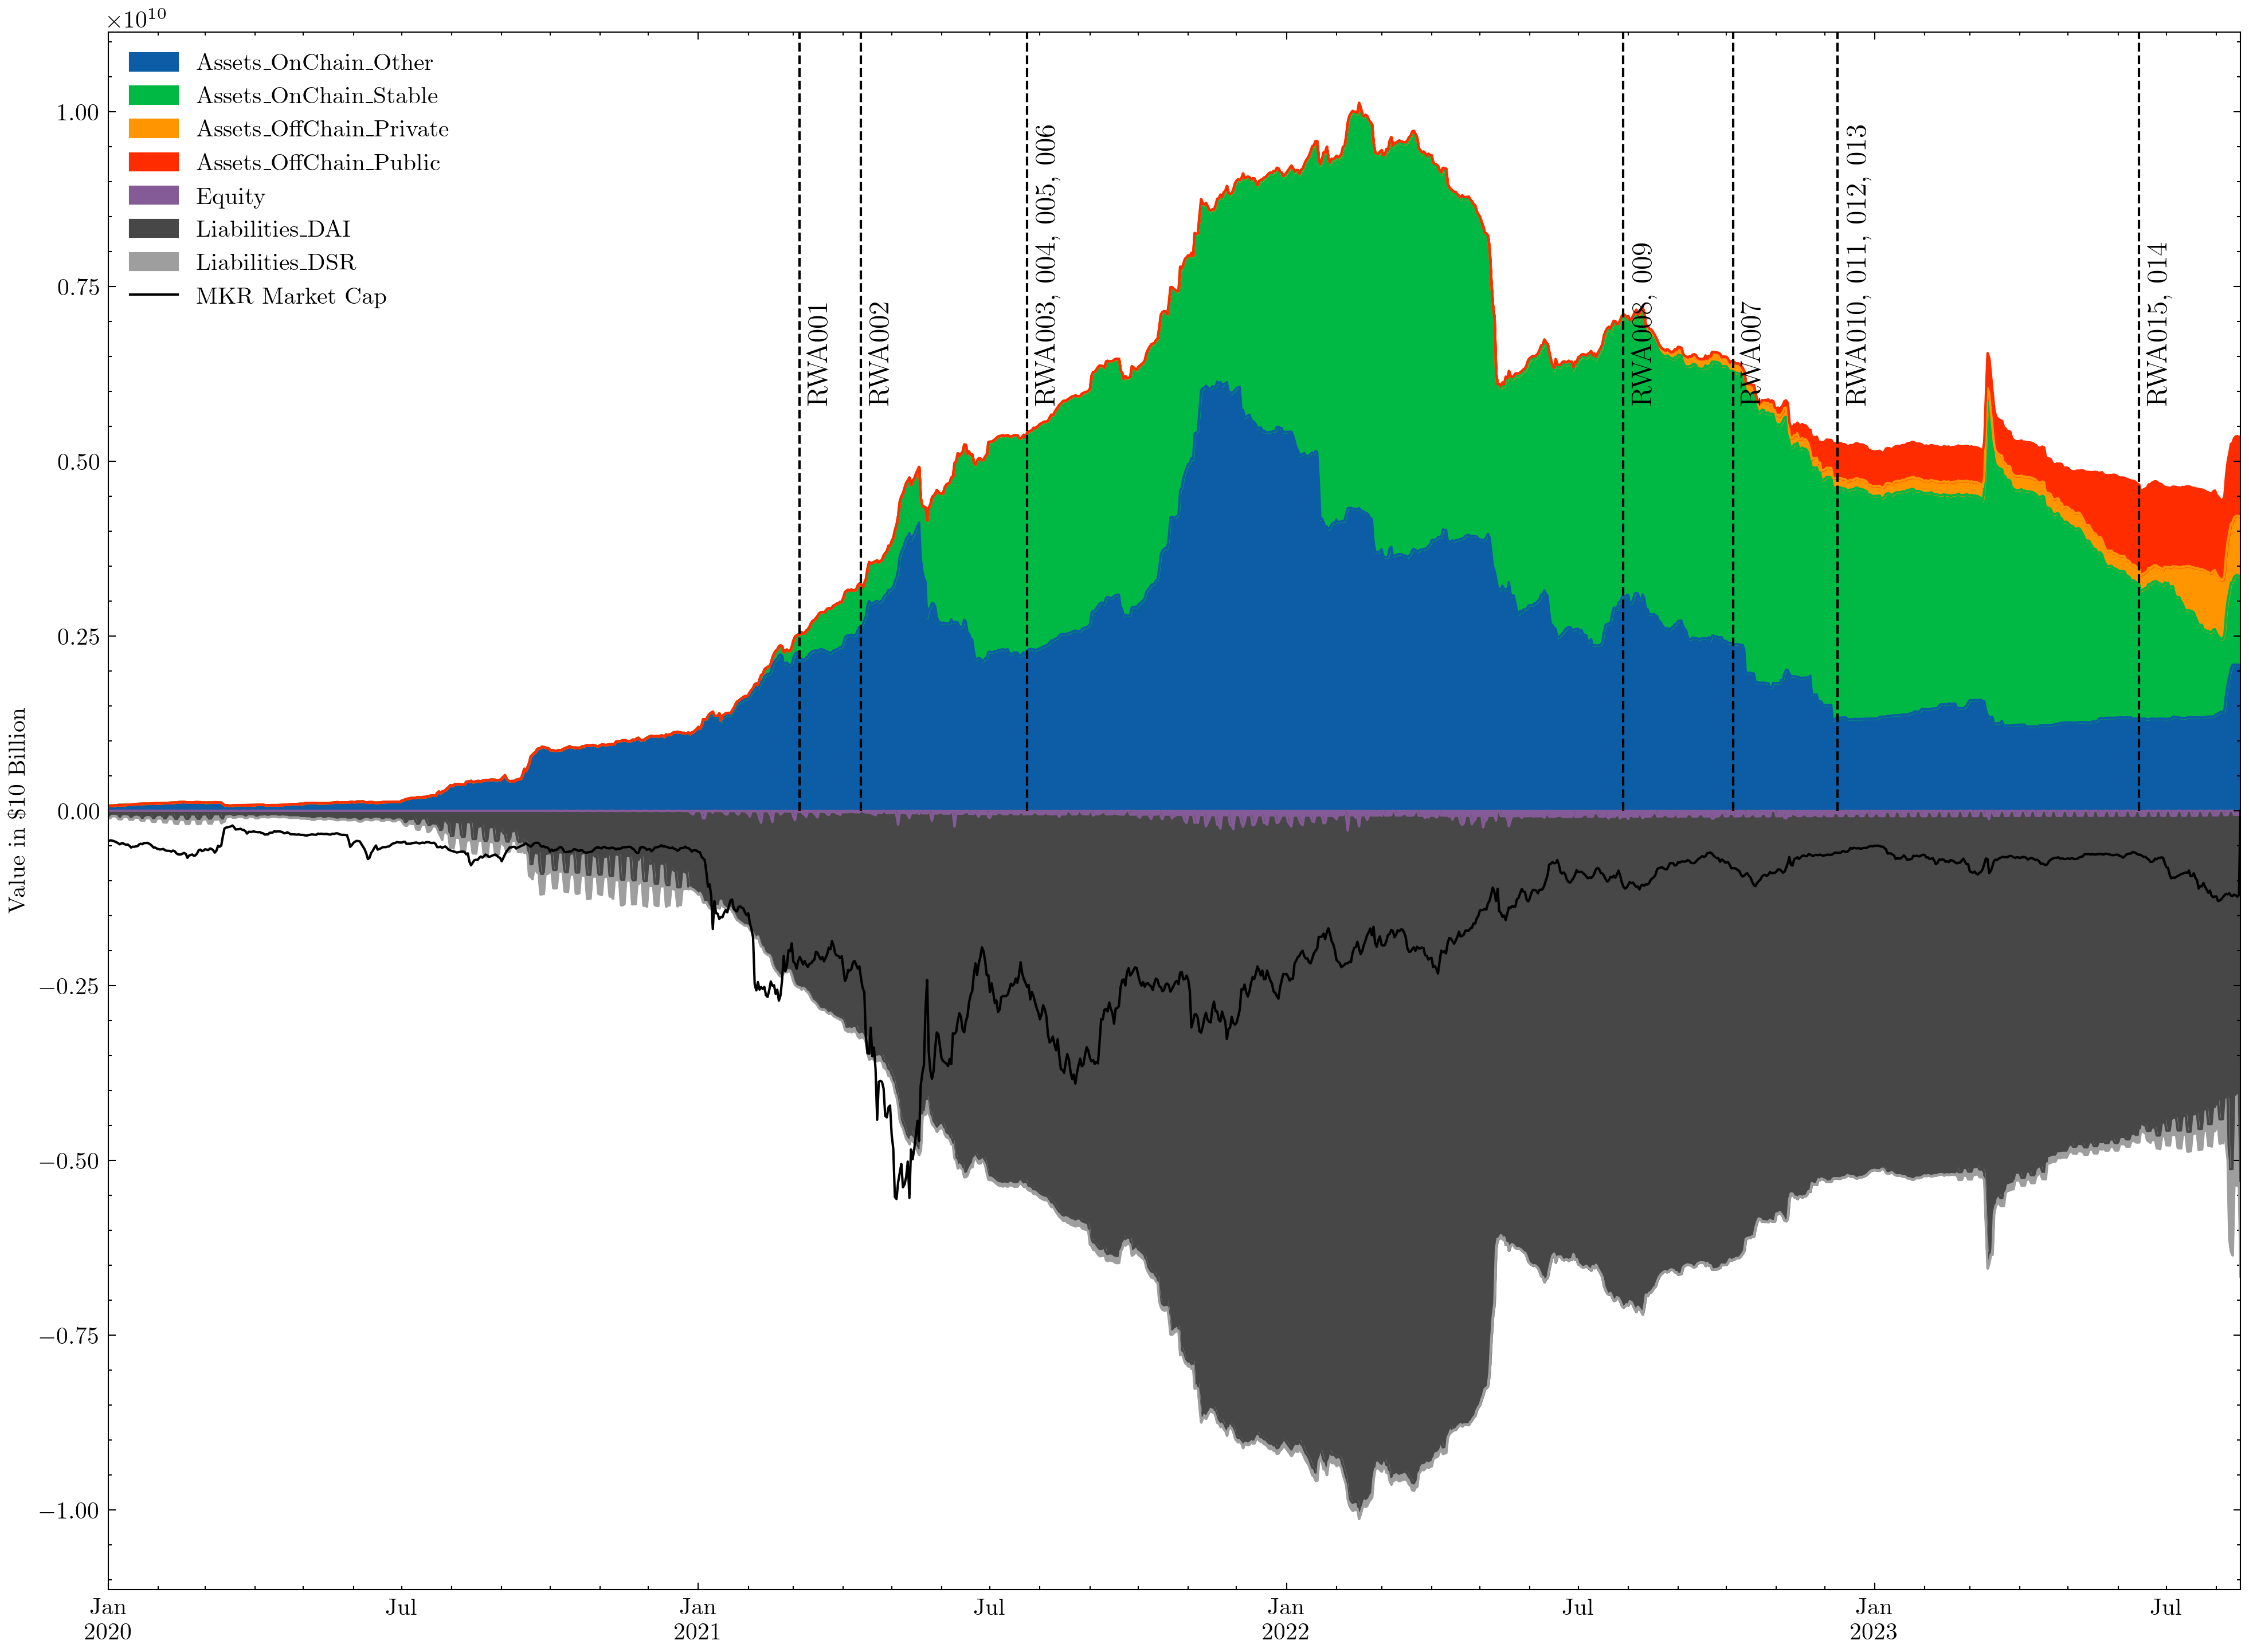
\includegraphics[width=90mm]{Figs/historical_balancesheet_with_votes.png}
\caption{MakerDAO Balance Sheet, 2020-2023}
\label{fig1}
\end{figure}
\end{frame}

\begin{frame}{Appendix: Some System Components}
\begin{figure}
\centering
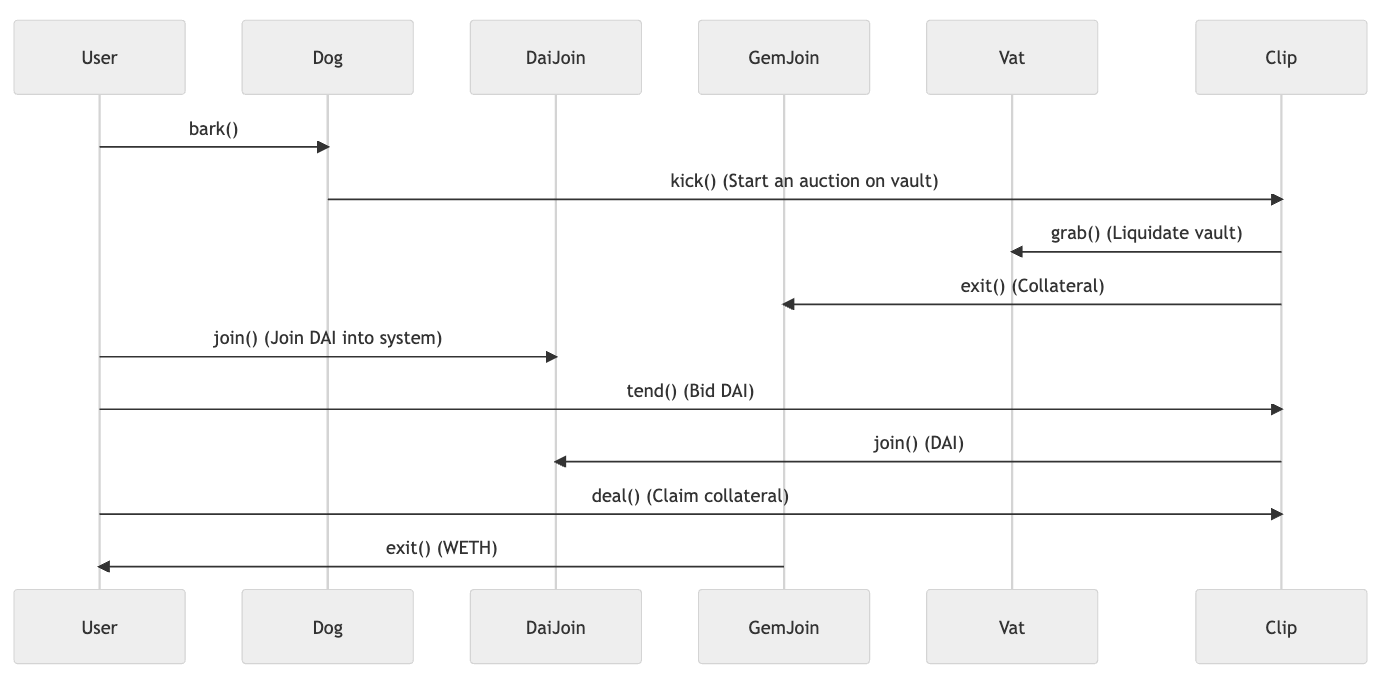
\includegraphics[width=100mm]{resources/system.png}
\caption{Simplified System Components of MakerDAO}
\label{fig2}
\end{figure}
\end{frame}

\begin{frame}{Appendix: Formal Design of Method}
\begin{schema}{Kick}
\Delta Clipper \\
tab: \real \\
lot: \real \\
% usr: USER \\
kpr: \seq CHAR \\
now: \nat \\
\where
tab > 0 \\
lot > 0 \\
kicks' = kicks + 1 \\
ACTIVE' = active \cup \{kicks'\} \\
\end{schema}

% \vspace{1cm}  % Add some space between the schema and the caption
\centering
\normalsize{Schema: Begin Collateral Auction}
\vfill  % Fill the remaining space to push the caption towards the bottom
\end{frame}


\begin{frame}{Appendix: Global Interactive Sensitivity}
\begin{figure}
\centering
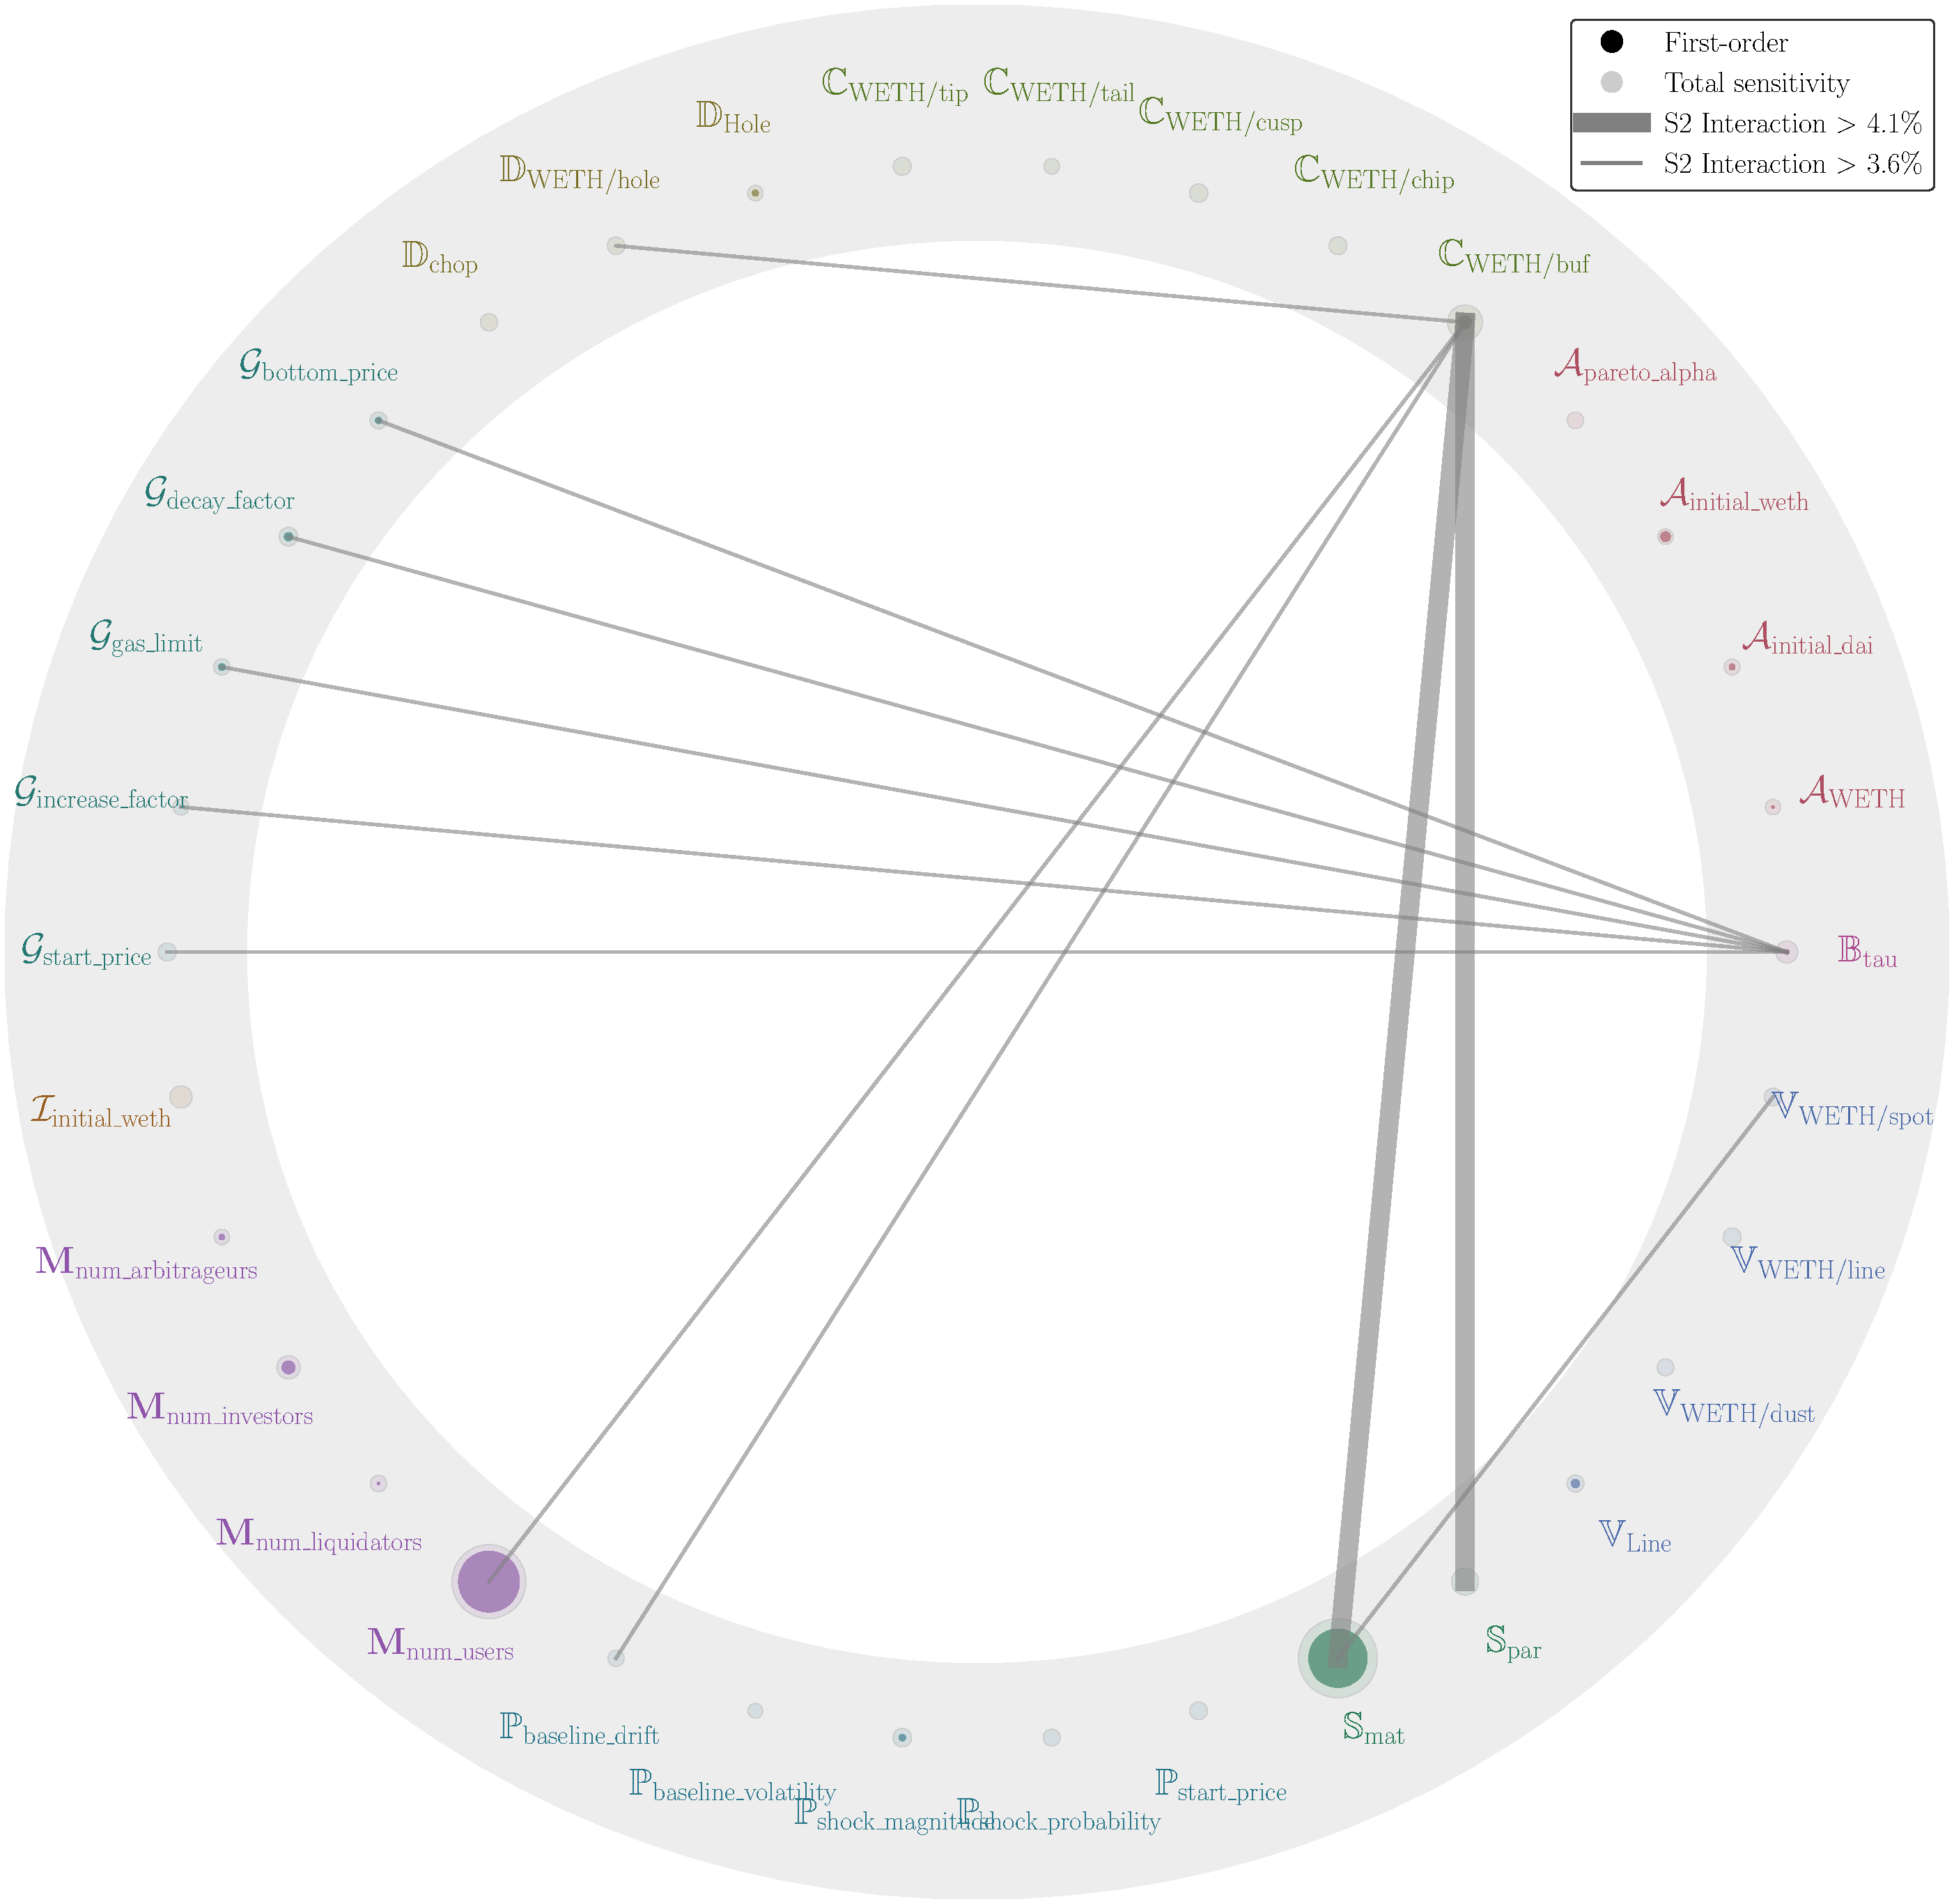
\includegraphics[width=70mm]{Figs/Sobol' Sensitivity Analysis, 35840 model runs.pdf}
\caption{Global Sensitivity Analysis, 35840 model runs}
\label{fig3}
\end{figure}
\end{frame}

\begin{frame}{Appendix: Time series Sensitivity}
\begin{figure}
\centering
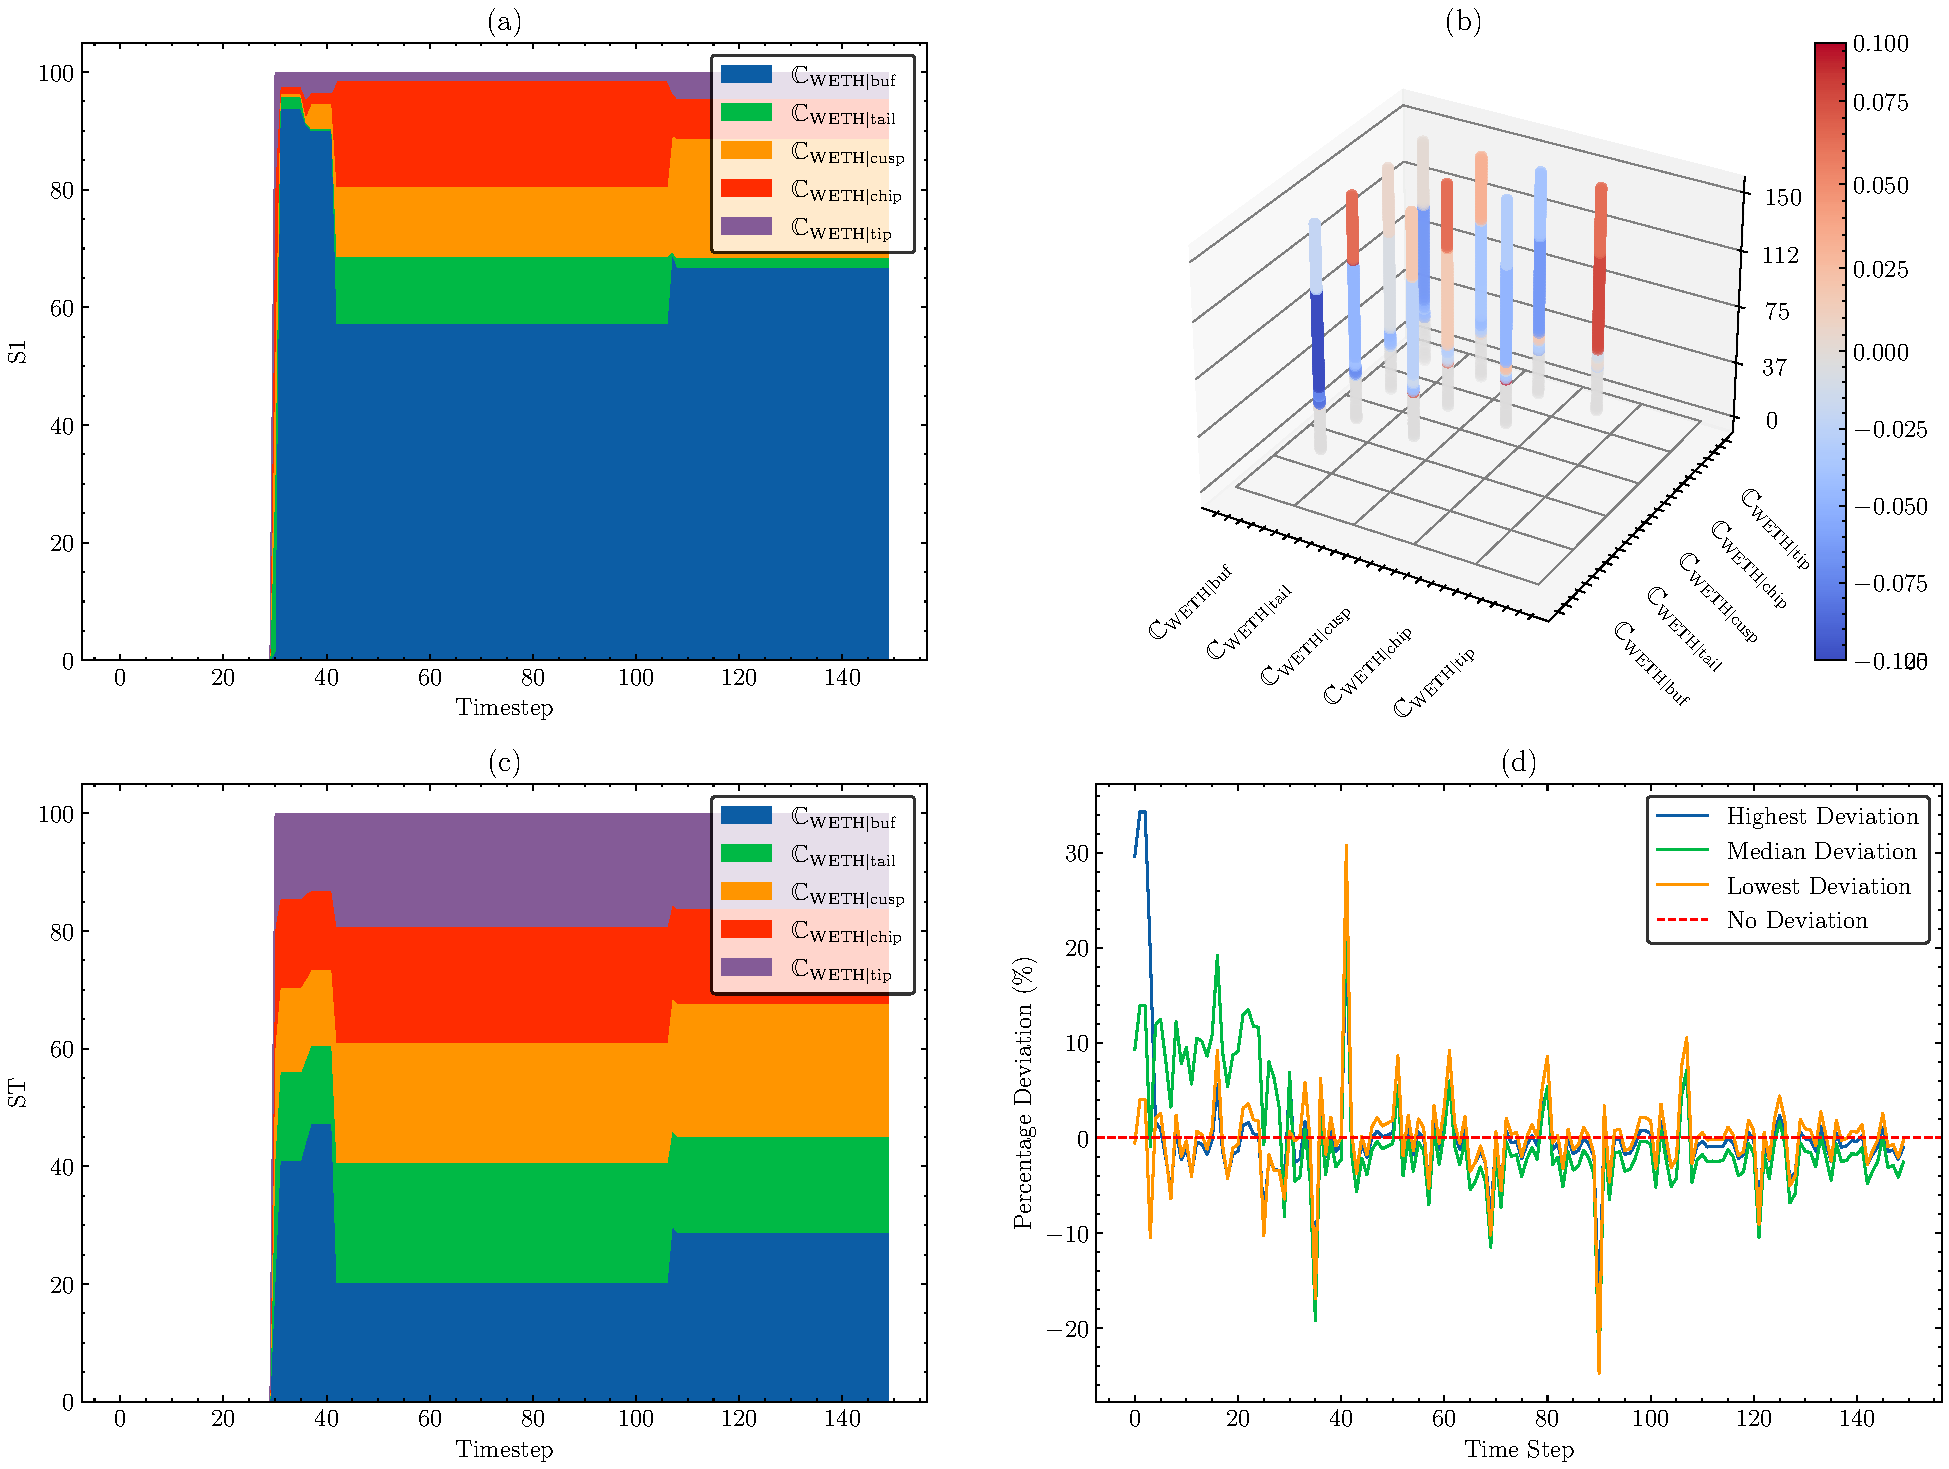
\includegraphics[width=85mm]{Figs/SOBOL_time_series_for_problem_cliplike_n10.pdf}
\caption{Sensitivity Analysis for Auction Parameters, 10240 Model Runs}
\label{fig4}
\end{figure}
\end{frame}

\end{document}
